\documentclass{article}%
\usepackage[T1]{fontenc}%
\usepackage[utf8]{inputenc}%
\usepackage{lmodern}%
\usepackage{textcomp}%
\usepackage{lastpage}%
\usepackage{graphicx}%
%
\title{2014 Fowler et al\_ This is an open{-}access article distribute}%
\author{\textit{Ting Da{-}Xia}}%
\date{08-06-2002}%
%
\begin{document}%
\normalsize%
\maketitle%
\section{I’ve written in the past about this issue of open{-}access}%
\label{sec:Ivewritteninthepastaboutthisissueofopen{-}access}%
I’ve written in the past about this issue of open{-}access. I’m happy to do so in because it provides a useful option for those who want to extend the freedom of information or debate free from censorship and for those who simply want to view information in its full view without being subjected to its banning by the government. They are obliged to carry a warrant for that information which potentially would be scrutinised by other scholars, without their knowledge and vetting by government officials.\newline%
I’m not sure that the Computer Fraud and Abuse Act will stand in the way of such an open access format. The gag order against Apple Apple came after a trial in which a court threw out the suit; however, this is a different situation in which publishers and editors of large publishing houses have to apply the following requirements for their access to available information:\newline%
Given your organisation’s high volume of international editions and the failure of the digital publishing industry to develop a code of ethics and express standards to reflect them, a ruling in the Federal Court would not impose wider restrictions for publishing by other media.\newline%
If open access is one of those strict guidelines, then you want to have a discussion with readers and use those limits to assess your position. One of the things they could do is provide title descriptions or extract short form versions of items in paragraphs that you typically publish. There are better options, and some can be considerably simpler (a full list of good, easy{-}to{-}read titles can be found here).\newline%
If open access is a new material which your organisation is looking to publish, be sure you have the right legal documents in mind when publishing it. I’ve used the NSS page to print results of my ISO 9001 certification. A copy is available here, e, by e for £11.49.\newline%

%


\begin{figure}[h!]%
\centering%
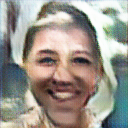
\includegraphics[width=120px]{./photos_from_epoch_8/samples_8_242.png}%
\caption{a man wearing a tie and a shirt .}%
\end{figure}

%
\end{document}